\documentclass[11pt, oneside]{article}   	
\usepackage{geometry}                    		
\usepackage{graphicx}			
\usepackage{amssymb,amsmath,amsthm}
\usepackage{tikz}
\usepackage{enumerate}
\usepackage{mathtools}
\usepackage[symbol]{footmisc}
\usepackage{xcolor}
\usepackage{titlesec}
\usepackage{tabularx}
\usepackage[linesnumbered,ruled]{algorithm2e}
\usepackage{pifont}
\usepackage{colortbl}
\usepackage[most]{tcolorbox}
\usepackage{setspace}
\usepackage{listings}
\usepackage[T1]{fontenc}
\usepackage[scaled]{beramono}
% fancy font
\usepackage{mathpazo}
\usepackage{eulervm}
\doublespacing

\geometry{
a4paper,
total={190mm,257mm},
left=10mm,
top=10mm,
}

\lstset{
  language=Python,
  showstringspaces=false,
  formfeed=\newpage,
  tabsize=4,
  commentstyle=\itshape,
  basicstyle=\ttfamily,
  morekeywords={models, lambda, forms}
}

\newcommand{\code}[2]{
  \hrulefill
  \subsection*{#1}
  \lstinputlisting{#2}
  \vspace{2em}
}

\newcommand\bb[1]{\mathbb{#1}}
\renewcommand\cal[1]{\mathcal{#1}}
\renewcommand\bf[1]{\textbf{#1}}
\newcommand\myeq{\stackrel{\mathclap{\normalfont\mbox{\tiny\sffamily def}}}{=}}
\renewcommand{\thefootnote}{\fnsymbol{footnote}}
% \snode{ID}{NUMBER} becomes \node{ID}[item]{\ensuremath{NUMBER}}
\newcommand{\snode}[2]{\node(#1)[item]{\ensuremath{#2}}}
% \nodelabel{SUBSCRIPT} becomes \node[label]{\ensuremath{S_SUBSCRIPT}}
\newcommand{\nodelabel}[1]{\node[label]{\ensuremath{S_#1}}}
\newcommand{\cmark}{\ding{51}}%
\newcommand{\xmark}{\ding{55}}%


\definecolor {processblue}{cmyk}{0.3,0,0,0}
\definecolor {grey}{cmyk}{0,1,0,1}
\usetikzlibrary{shapes,positioning,calc,chains}
\usetikzlibrary{mindmap,trees}
\usetikzlibrary{plotmarks}
\usetikzlibrary{matrix}
\usetikzlibrary{arrows,automata}
% Make automata look nice
\tikzset{
  ->, >=stealth', shorten >=1pt, semithick,
  auto, node distance=6em,
  every state/.style={draw=black!50,very thick,fill=black!20},
  initial text=$ $
}

\everymath{\displaystyle}
\titleformat*{\section}{\LARGE\bfseries}
\titleformat*{\subsection}{\Large\bfseries}
\titleformat*{\subsubsection}{\large\bfseries}
\titleformat*{\paragraph}{\large\bfseries}
\titleformat*{\subparagraph}{\large\bfseries}
\title{Assignment 01}
\author{Question 01}
\date{ Shuheng Cao}							


\begin{document}
\thispagestyle{empty}
\def\layersep{2.5cm}
\nopagecolor
% \begin{tikzpicture}[shorten >=1pt,->,draw=black!50, node distance=\layersep]
%     \tikzstyle{every pin edge}=[<-,shorten <=1pt]
%     \tikzstyle{neuron}=[circle,fill=black!25,minimum size=17pt,inner sep=0pt]
%     \tikzstyle{input neuron}=[neuron, fill=green!50, draw=white, ultra thick, fill opacity=0];
%     \tikzstyle{output neuron}=[neuron, fill=red!50, draw=white, ultra thick, fill opacity=0];
%     \tikzstyle{hidden neuron}=[neuron, fill=blue!50, draw=white, ultra thick, fill opacity=0];
%     \tikzstyle{annot} = [text width=6em, text centered, color = white]


% 		\node[inner sep=0pt] (R) at (0,-2.5) {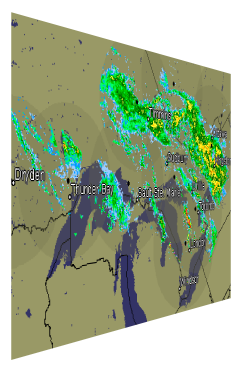
\includegraphics[width=1cm]{example}};

%     % Draw the input layer nodes
%     \foreach \name / \y in {1,...,4}
%     % This is the same as writing \foreach \name / \y in {1/1,2/2,3/3,4/4}
%         % \node[input neuron, pin=left:Input \#\y] (I-\name) at (0,-\y) {};
%         \node[input neuron] (I-\name) at (\layersep,-\y) {};

%     % Draw the hidden layer nodes
%     \foreach \name / \y in {1,...,5}
%         \path[yshift=0.5cm]
% 						\node[hidden neuron] (H-\name) at (2 * \layersep,-\y cm) {};
						
		

% 		% Draw the hidden layer nodes
%     \foreach \name / \y in {1,...,5}
%         \path[yshift=0.5cm]
%             \node[hidden neuron] (X-\name) at (3 * \layersep,-\y cm) {};

%     % Draw the output layer node
%     \node[output neuron,pin={[pin edge={->}]right:Output}, right of=X-3] (O) {};

%     % Connect every node in the input layer with every node in the
% 		% hidden layer.
% 		\foreach \dest in {1,...,4}
% 				\path (R) edge (I-\dest);

%     \foreach \source in {1,...,4}
%         \foreach \dest in {1,...,5}
%             \path (I-\source) edge (H-\dest);

% 		\foreach \source in {1,...,6}
% 				\foreach \dest in {1,...,5}
% 						\path (H-\source) edge (X-\dest);
%     % Connect every node in the hidden layer with the output layer
%     \foreach \source in {1,...,5}
%         \path (X-\source) edge (O);

%     % Annotate the layers
% 		\node[annot,above of=H-1, node distance=1cm] (h1) {MP layer};
%     \node[annot,right of=h1] (h2) {Hidden layer};
%     \node[annot,left of=h1] {Conv layer};
%     \node[annot,right of=h2] {Output};
% \end{tikzpicture}

\begin{tikzpicture}[shorten >=1pt,->,draw=black!50, node distance=\layersep]
	\tikzstyle{every pin edge}=[<-,shorten <=1pt]
	\tikzstyle{neuron}=[circle,fill=black!25,minimum size=17pt,inner sep=0pt]
	\tikzstyle{input neuron}=[neuron, fill=green!50, draw=white, ultra thick, fill opacity=0];
	\tikzstyle{output neuron}=[neuron, fill=red!50, draw=white, ultra thick, fill opacity=0];
	\tikzstyle{hidden neuron}=[neuron, fill=blue!50, draw=white, ultra thick, fill opacity=0];
	\tikzstyle{annot} = [text width=6em, text centered, color = white]


	\node[inner sep=0pt] (R) at (0,-4) {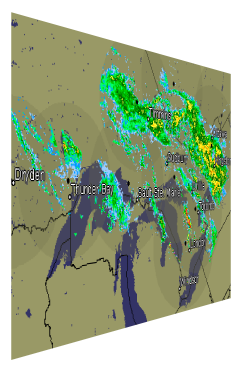
\includegraphics[width=1cm]{example}};

    % Draw the input layer nodes
    \foreach \name / \y in {1,...,8}
    % This is the same as writing \foreach \name / \y in {1/1,2/2,3/3,4/4}
        % \node[input neuron, pin=left:Input \#\y] (I-\name) at (0,-\y) {};
        \node[input neuron, fill opacity=1, fill=green!40!black] (I-\name) at (\layersep,-\y) {};

		
    % Draw the hidden layer nodes
    \foreach \name / \y in {1,...,6}
        \path[yshift=0.5cm]
            node[hidden neuron, fill opacity=1, fill=green!40!black] (H-\name) at (2 * \layersep,-\y cm) {};
						
		

		% Draw the hidden layer nodes
    \foreach \name / \y in {1,...,4}
        \path[yshift=0.5cm]
            node[hidden neuron, fill opacity=1, fill=green!40!black] (X-\name) at (3 * \layersep,-\y cm) {};

		
		\foreach \name / \y in {6,...,8}
				\path[yshift=0.5cm]
						node[hidden neuron, pin=left:, fill opacity=1, fill=green!40!black] (X-\name) at (3 * \layersep,-\y cm) {};
		
		


    % Draw the output layer node
    % \node[output neuron,pin={[pin edge={->}]right:Output}, right of=X-3] (O) {};
    % \node[output neuron] (O) at (5 * \layersep,-4) {};
		\foreach \name / \y in {1,...,8}
				\path[yshift=0.5cm]
						node[hidden neuron, fill opacity=1, fill=green!40!black] (Y-\name) at (4 * \layersep,-\y cm) {};

		\foreach \name / \y in {3,...,6}
				\path[yshift=0.5cm]
						node[hidden neuron, pin={[pin edge={->}]right:}, fill opacity=1, fill=green!40!black] (O-\name) at (5 * \layersep,-\y cm) {};
    % Connect every node in the input layer with every node in the
		% hidden layer.
		\foreach \dest in {1,...,8}
				\path (R) edge (I-\dest);

    \foreach \source in {1,...,4}
        \foreach \dest in {1,...,3}
            \path (I-\source) edge (H-\dest);


    \foreach \source in {5,...,8}
				\foreach \dest in {4,...,6}
						\path (I-\source) edge (H-\dest);
						
		\foreach \source in {1,...,6}
				\foreach \dest in {1,...,4}
						\path (H-\source) edge (X-\dest);
    % Connect every node in the hidden layer with the output layer
    \foreach \source in {1,...,4}
				\foreach \dest in {1,...,8}
						\path (X-\source) edge (Y-\dest);
		
		\foreach \source in {6,...,8}
				\foreach \dest in {1,...,8}
						\path (X-\source) edge (Y-\dest);

		\foreach \source in {1,...,8}
				\foreach \dest in {3,...,6}
						\path (Y-\source) edge (O-\dest);
    % Annotate the layers
    \node[annot,above of=H-1, node distance=1cm] (h1) {Pool layers};
    \node[annot,right of=h1] (h2) {FC layer};
    \node[annot,left of=h1] {Conv layers};
		\node[annot,right of=h2] (h3) {Hidden layer};
		\node[annot,right of=h3] {Outputs};
\end{tikzpicture}

\end{document}.


% Useful tricks:
% ********************************** Mind Map *************************************
% \begin{figure}[!h]
	% 	\resizebox{\textwidth}{!}{
	% 	\begin{tikzpicture}[
		% 		mindmap,
		% 		grow cyclic, text width=4cm, align=center,
		% 		every node/.style={concept},
		% 		concept color=black!80, text = white ,font=\linespread{1.8}\selectfont,
		% 		%root/.style= {concept color=black!40,font=\large\bfseries,text width=12em},
		% 		level 1/.style={level distance=8cm,sibling angle=72},
		% 		level 2/.style={level distance=6cm,sibling angle=80},
		% 		level 3/.style={level distance=6cm,sibling angle=45}]
		
		%     \node [root concept, scale=1.5] {\textbf{\Large{Midterm \\ Review}}}
		%     child [concept color=black!60] { node {\huge{Decision\\ Tree}}	
		%     child [concept color=black!40,style={level distance=6cm,sibling angle=80}] { node {\huge{Prove}}}
		%     child [concept color=black!40,style={level distance=6cm,sibling angle=80}]{ node {\huge{Disprove}}}
		%     }
		%     % child [concept color=green!30] { node {One concept}
		%     % 	child [concept color=green!40]{ node {description \\ of concept 1}}
		%     %    % child { node {B}}
		%     % }
		%     child [concept color=black!60] { node {\Large{Non-comparison \\Based Sorting}}
		%     child [concept color=black!40] { node {\huge{Bucket Sort}}}
		%     child [concept color=black!40] { node {\huge{Count Sort}}}
		%     child [concept color=black!40] { node {\huge{Radix Sort}}}
		%     }
		%     child [concept color=black!60] { node {\huge{Randomized\\ Algorithm}}
		%     child[concept color=black!40,style={level distance=6cm,sibling angle=80}] {node {\huge{Quick Sort}}}
		%     child[concept color=black!40,style={level distance=6cm,sibling angle=80}] {node {\huge{Quick Select}}}
		%     }
		%     child [concept color=black!60]  { node {\huge{Binary\\ Heap}}
		%     % child[concept color=black!40] { node {\huge{Notation}}}
		%     child[concept color=black!40] { node {\huge{\textit{fix-down}}}}
		%     child[concept color=black!40] { node {\huge{\textit{fix-up} }}}
		%     child[concept color=black!40] { node {\huge{\textit{heapify}  }}}
		%     }
		%     child [concept color=black!60]  { node {\LARGE{Asymptotic Analysis}}
		%     % child[concept color=black!40] { node {\huge{Notation}}}
		%     child[concept color=black!40] { node {\huge{\textit{Notation} }}}
		%     child[concept color=black!40] { node {\huge{\textit{Relationship}}}}
		%     };
	% 	\end{tikzpicture}}
	% 	% \caption{Outline}
% \end{figure}

% ********************************** Fancy Table **********************************
% \newcolumntype{M}[1]{>{\centering\arraybackslash}m{#1}}
% \newcolumntype{N}{@{}m{0pt}@{}}
% \begin{figure}[ht]
	% 	\begin{center}
		% 		\begin{tabular}{|M{3cm}|M{3cm}||M{0.75cm}|M{0.75cm}|M{0.75cm}|M{0.75cm}|M{0.75cm}|N} \hline
			% 			$f(n)$ & $g(n)$ &  $o$ &  $O$ &  $\omega$ & $\Omega$ & $\Theta$&  \\ [3mm]\hline \hline
			% 			$n^{2}+\log^{10}{n}$& $n^{2} + \log{n}$& & & & & \\[3mm] \hline
			% 			$2^{n}$&$3^{n}$ & & & & & \\[3mm] \hline
			% 			$n\cdot\log{n}$&$\log{\left (n^{2n}\right )}$ & & & & & \\[3mm] \hline
			% 			$n^{n}$&$n^{\frac{n}{2}}$ & & & & &  \\[3mm] \hline
		% 		\end{tabular}
	% 	\end{center}
% \end{figure}

% ********************************** Pseudo Code **********************************
% \begin{figure}[ht]
% 	\centering
% 	\begin{minipage}{.8\linewidth}
% 		\begin{algorithm}[H]
% 			\DontPrintSemicolon
% 			\SetKwFunction{FMain}{search}
% 			\SetKwProg{Fn}{Function}{:}{}
% 			\Fn{\FMain{$T_0$, $T_1$, $key$}}{
% 			\textbf{Input: }$T_0$ and $T_2$ are two hash tables of size $M$ that comes with two independent hash functions $h_{0}$ and $h_{1}$\;
% 			$candidate_0 \gets h_0(key)$\;
% 			$candidate_1 \gets h_1(key)$\;
% 			\uIf{$T_0[candidate_0].key = key$}{\Return $T_0[candidate_0]$}\uElseIf{$T_1[candidate_1].key = key$}{\Return $T_1[candidate_1]$}\Else{\Return \textit{not found}\;}
% 			}
% 			\SetKwFunction{FMain}{insert}
% 			\SetKwProg{Fn}{Function}{:}{}
% 			\Fn{\FMain{$T_0$, $T_1$, $key$}}{
% 			\For{$i \gets 0$ \KwTo $2M$ }{
% 			$cur \gets i \mod{2}$\;
% 			\If{$T_{cur}\left[	h_{cur}(key)	\right]$ is empty}{
% 			$T_{cur}\left[	h_{cur}(key)	\right] \gets key$\;
% 			\Return
% 			}
% 			\textit{swap}$\left(T_{cur}\left[	h_{cur}(key)	\right], key\right)$\;
% 			}
% 			\textit{reshuffle}($T$)\;
% 			\textit{insert}($T_0$, $T_1$, $key$) \;
% 			}\;
% 			\SetKwFunction{FMain}{delete}
% 			\SetKwProg{Fn}{Function}{:}{}
% 			\Fn{\FMain{$T_0$, $T_1$, $key$}}{
% 			$res\gets$ \textit{search}($T_0$, $T_1$, $key$)\;
% 			delete($res$)\;
% 			}
% 			\caption{Cuckoo Hashing}
% 		\end{algorithm}
% 	\end{minipage}
% \end{figure}



% ********************************** Normal Tree **********************************
% \begin{center}
	% 	\begin{tikzpicture}
		% 		[every node/.style={draw,minimum width={10mm}}, 
		% 		level 1/.style={sibling distance=50mm},
		% 		level 2/.style={sibling distance=20mm},
		% 		level 3/.style={sibling distance=15mm}]
		% 		\node [circle, draw, minimum width={10mm}] at (6, 0)  {4}
		% 		child{node [circle, draw]  {2}
		% 		child{node [circle,draw]  {1}}
		% 		child{node [circle, draw]  {3}}
		% 		}
		% 		child{node [circle, draw]  {9}
		% 		child{node [circle,draw]  {6}
		% 		child{node[circle,draw] {5}}
		% 		child{node[circle,draw]  {8}}
		% 		}
		% 		child{node [circle, draw]  {10}}
		% 		}
		% 		;
	% 	\end{tikzpicture}\quad
	% 	\begin{tikzpicture}
		% 		[every node/.style={draw,minimum width={10mm}}, 
		% 		level 1/.style={sibling distance=50mm},
		% 		level 2/.style={sibling distance=20mm},
		% 		level 3/.style={sibling distance=15mm}]
		% 		\node [circle, draw, minimum width={10mm}] at (6, 0)  {}
		% 		child{node [circle, draw]  {}
		% 		child{node [circle,draw]  {}}
		% 		child{node [circle, draw]  {}}
		% 		}
		% 		child{node [circle, draw]  {}
		% 		child{node [circle,draw]  {}
		% 		child{node[circle,draw] {}}
		% 		child{node[circle,draw]  {}}
		% 		}
		% 		child{node [circle, draw]  {}}
		% 		}
		% 		;
	% 	\end{tikzpicture}
% \end{center}

% ********************************** Split Tree / Minipage Example ****************
% \begin{figure}[ht]
	% 	\begin{minipage}{0.5\linewidth}
		% 		\centering
		% 		\begin{tikzpicture}
			% 			[every node/.style = {draw, shape = circle split, grow = down,minimum width={10mm}},
			% 			level 1/.style={sibling distance=35mm},
			% 			level 2/.style={sibling distance=20mm},
			% 			level 3/.style={sibling distance=15mm}]
			% 			\node(z){0\nodepart{lower}}
			% 			child{
			% 			node{-3\nodepart{lower}}
			% 			child{node {-5\nodepart{lower}}
			% 			child{node {-6\nodepart{lower}}
			% 			child{node {-7\nodepart{lower}}}
			% 			child [missing]
			% 			}
			% 			child{node {-4\nodepart{lower}}}
			% 			}
			% 			child{node {-2\nodepart{lower}}
			% 			child [missing]
			% 			child{node {-1\nodepart{lower}}}
			% 			}
			% 			}
			% 			child{
			% 			node{2\nodepart{lower}}
			% 			child{node {1\nodepart{lower}}}
			% 			child{node {3\nodepart{lower}}
			% 			child [missing]
			% 			child{node {4\nodepart{lower}}}
			% 			}
			% 			};
		% 		\end{tikzpicture}
	% 	\end{minipage}
	% 	\begin{minipage}{0.5\linewidth}
		% 		$(1)$ Perform \textit{insert}$(-8)$ on the AVL tree.
		% 		\vspace{70mm}
	% 	\end{minipage}
% \end{figure}

% ********************************** Skip List ************************************
% \begin{center}
	% 	\begin{tikzpicture}[
		% 		start chain,
		% 		every node/.style={font=\small},
		% 		item/.style={rectangle,minimum height=6mm,minimum width=7mm,
		% 		rounded corners=2mm,thick,draw=black},
		% 		label/.style={rectangle,minimum size=6mm}
		% 		]
		
		% 		% The nodes of the skip list are drawn in a matrix
		% 		% \\ delimits the rows while & delimits the columns
		% 		\matrix[row sep=3mm, column sep=5mm]{
		% 		% Row 5: -infty ... +infty
		% 		\nodelabel{5}; & \snode{5a}{-\infty}; && & && && & &&   & && \snode{5n}{+\infty};\\
		
		
		% 		% Row 4: -infty ... +infty
		% 		\nodelabel{4}; & \snode{4a}{-\infty};& & & &&& & &\snode{4i}{27};&  & &&  & \snode{4n}{+\infty};\\
		
		% 		% Row 3: -infty ... +infty
		% 		\nodelabel{3}; & \snode{3a}{-\infty};& && & & &&& \snode{3i}{27}; & &  & \snode{3l}{66}; && \snode{3n}{+\infty};\\
		
		% 		% Row 2: -infty ...  ... +infty
		% 		\nodelabel{2}; & \snode{2a}{-\infty};& & \snode{2c}{8}; && & \snode{2f}{18}; & \snode{2g}{21}; 
		% 		& & \snode{2i}{27};&&    & \snode{2l}{66}; && \snode{2n}{+\infty};\\
		
		% 		% Row 1: -infty ...  ... +infty
		% 		\nodelabel{1}; & \snode{1a}{-\infty};&\snode{1b}{4}; & \snode{1c}{8}; & \snode{1d}{16}; & \snode{1e}{17}; & \snode{1f}{18}; & \snode{1g}{21}; 
		% 		& \snode{1h}{22};& \snode{1i}{27}; & \snode{1j}{28}; &  & \snode{1l}{66};& \snode{1m}{99}; & \snode{1n}{+\infty};\\
		
		% 		% Row 0: -infty 4  8   16  17  18  21 22  27  28  42  66 99 +infty
		% 		\nodelabel{0}; & \snode{0a}{-\infty}; &\snode{0b}{4};	& \snode{0c}{8};  & \snode{0d}{16};  & \snode{0e}{17}; & \snode{0f}{18}; & \snode{0g}{21}; 
		% 		& \snode{0h}{22};& \snode{0i}{27};  & \snode{0j}{28};& \snode{0k}{42};  & \snode{0l}{66};& \snode{0m}{99};  & \snode{0n}{+\infty};\\
		% 		};
		
		% 		% Start chaining the nodes together
		% 		{
		% 		% Horizontal chains
		% 		% Specify a starting node (by ID), and join to other nodes (by going "through" them in an unbroken line)
		% 		% Eg row 2: Start at 2a, join 2e, join 2h, join 2i
		% 		[start chain] \chainin(0a); \chainin(0b) [join]; \chainin(0c) [join]; \chainin(0d) [join]; \chainin(0e) [join]; \chainin(0f) [join];\chainin(0g) [join]; \chainin(0h) [join];\chainin(0i) [join];
		% 		\chainin(0j) [join];\chainin(0k) [join]; \chainin(0l) [join]; \chainin(0m) [join]; \chainin(0n) [join];
		% 		[start chain] \chainin(1a); \chainin(1b) [join]; \chainin(1c) [join]; \chainin(1d) [join]; \chainin(1e) [join]; \chainin(1f) [join];\chainin(1g) [join]; \chainin(1h) [join];\chainin(1i) [join];
		% 		\chainin(1j) [join]; \chainin(1l) [join]; \chainin(1m) [join]; \chainin(1n) [join];       
		% 		[start chain] \chainin(2a); \chainin(2c) [join]; \chainin(2f) [join];\chainin(2g) [join];\chainin(2i) [join]; \chainin(2l) [join]; \chainin(2n) [join];
		% 		[start chain] \chainin(3a); \chainin(3i) [join];\chainin(3l) [join]; \chainin(3n) [join];
		% 		[start chain] \chainin(4a); \chainin(4i) [join];\chainin(4n) [join];
		% 		[start chain] \chainin(5a); \chainin(5n) [join];
		% 		}
		% 		{
		% 		% Vertical chains
		% 		% Need to be separate chains from the horizontal ones
		% 		[start chain] \chainin(0a); \chainin(1a) [join]; \chainin(2a) [join]; \chainin(3a) [join]; \chainin(4a) [join]; \chainin(5a) [join]; 
		% 		[start chain] \chainin(0b); \chainin(1b) [join]; 
		% 		[start chain] \chainin(0c); \chainin(1c) [join]; \chainin(2c) [join];
		% 		[start chain] \chainin(0d); \chainin(1d) [join]; 
		% 		[start chain] \chainin(0e); \chainin(1e) [join]; 
		% 		[start chain] \chainin(0f); \chainin(1f) [join]; \chainin(2f) [join];
		% 		[start chain] \chainin(0g); \chainin(1g) [join]; \chainin(2g) [join];
		% 		[start chain] \chainin(0h); \chainin(1h) [join]; 
		% 		[start chain] \chainin(0i); \chainin(1i) [join]; \chainin(2i) [join]; \chainin(3i) [join]; \chainin(4i) [join];
		% 		[start chain] \chainin(0j); \chainin(1j) [join]; 
		% 		[start chain] \chainin(0l); \chainin(1l) [join]; \chainin(2l) [join]; \chainin(3l) [join];
		% 		[start chain] \chainin(0m); \chainin(1m) [join]; 
		% 		[start chain] \chainin(0n); \chainin(1n) [join]; \chainin(2n) [join]; \chainin(3n) [join]; \chainin(4n) [join]; \chainin(5n) [join]; 
		
		% 		}
	% 	\end{tikzpicture}
% \end{center}

% ********************************** Colored Tree *********************************
% \begin{center}
	% 	% define how to draw nodes and what distances to keep between them
	% 	\tikzset{
	% 	head/.style = {fill = green!60,
	% 	label = center:\textsf{\Large \xmark}},
	% 	tail/.style = {fill = white, text = black,
	% 	label = center:\textsf{\Large \cmark }}
	% 	}
	% 	\begin{tikzpicture}[
		% 		scale = 0.9, transform shape, thick,
		% 		every node/.style = {draw, circle, minimum size = 10mm},
		% 		grow = down,  % alignment of characters
		% 		level 1/.style = {sibling distance=10.3cm},
		% 		level 2/.style = {sibling distance=5.2cm}, 
		% 		level 3/.style = {sibling distance=2.5cm},
		% 		level 4/.style = {sibling distance=1.25cm}, 
		% 		level distance = 1.25cm
		% 		]
		% 		\node {\Large \cmark \par}
		% 		child { node [tail] (A) {}
		% 		child { node [tail] (B) {}
		% 		child { node [tail] {}
		% 		child { node [head] {}}
		% 		child { node [tail] {} }		     
		% 		}
		% 		child { node [tail] {} 
		% 		child { node [head] {}}
		% 		child { node [head] {} }		
		% 		}
		% 		}
		% 		child { node [tail] (C) {}
		% 		child { node [head] {}
		% 		child { node [fill = red!40] {\Large\xmark }}
		% 		child { node [fill = red!40] {\Large\xmark }}
		% 		}
		% 		child { node [tail] {} 
		% 		child { node [head] {}}
		% 		child { node [head] {}}
		% 		}
		% 		}
		% 		}
		% 		child { node [tail] (D) {}
		% 		child { node [head] (E) {}
		% 		child { node [fill = red!40]{\Large\xmark}
		% 		child { node [fill = red!40] {\Large\xmark }}					
		% 		child { node [fill = red!40] {\Large\xmark }}
		% 		}
		% 		child { node [fill = red!40] {\Large\xmark}
		% 		child { node [fill = red!40] {\Large\xmark }}					
		% 		child { node [fill = red!40] {\Large\xmark }}
		% 		}     
		% 		}
		% 		child { node [head] (F) {}
		% 		child { node [fill = red!40] {\Large\xmark}
		% 		child { node [fill = red!40] {\Large\xmark }}					
		% 		child { node [fill = red!40] {\Large\xmark }}				
		% 		}
		% 		child { node [fill = red!40] {\Large\xmark}
		% 		child { node [fill = red!40] {\Large\xmark }}					   	
		% 		}        
		% 		}
		% 		};
	% 	\end{tikzpicture}
% \end{center}

% ********************************** Tries ****************************************
% \begin{center}
	% 	\begin{tikzpicture}[level distance=1.5cm,
		% 		level 1/.style={sibling distance=3.5cm},
		% 		level 2/.style={sibling distance=3cm},
		% 		level 3/.style={sibling distance=2.5cm},
		% 		level 4/.style={sibling distance=2cm},
		% 		level 5/.style={sibling distance=1.5cm},
		% 		level 6/.style={sibling distance=1cm},]
		% 		\tikzstyle{every node}=[rectangle,draw,minimum size=0.001mm]
		% 		\node (Root) {0}
		% 		child {
		% 		node{1} 
		% 		child {node{2}
		% 		child{node{00\$} edge from parent node[left,draw=none] {\$} } 
		% 		child{node{0001\$} edge from parent node[left,draw=none] {0} } 
		% 		edge from parent node[left,draw=none] {0} }
		% 		child[missing]
		% 		child {node{2} 
		% 		child [level distance=3cm]{node{01001\$}
		% 		edge from parent node[left,draw=none] {0} 
		% 		}
		% 		child {
		% 		node{3}
		% 		child{node{011\$} edge from parent node[left,draw=none] {\$} }
		% 		child{node{01101\$} edge from parent node[left,draw=none] {0} }
		% 		edge from parent node[left,draw=none] {1} 
		% 		}
		% 		edge from parent node[left,draw=none] {1} 
		% 		}
		% 		edge from parent node[left,draw=none] {0} 
		% 		}
		% 		child [missing]
		% 		child [missing]
		% 		child {
		% 		node{1}
		% 		child {node{10\$}
		% 		edge from parent node[right,draw=none] {0} 	
		% 		}
		% 		child {
		% 		node{2} 
		% 		child{node{3} 
		% 		child{node{110\$}edge from parent node[right,draw=none] {\$} }
		% 		child{node{1101\$}edge from parent node[right,draw=none] {1} }		  	
		% 		edge from parent node[right,draw=none] {0} }
		% 		child{node{111\$} edge from parent node[right,draw=none] {1} }
		% 		edge from parent node[right,draw=none] {1} 
		% 		}
		% 		edge from parent node[right,draw=none] {1} 
		% 		};
	% 	\end{tikzpicture}
% \end{center}

% ********************************** 2D Plot **************************************
% \begin{center}
	% 	\begin{tikzpicture}[scale = 1.6]
		% 		\draw (0, 0) rectangle (8, 8);
		% 		\draw [red!50, dashed] (0,4) -- (8,4);
		% 		\draw [red!50, dashed] (4,0) -- (4,8);
		% 		\draw [green, dashed] (0,2) -- (4,2);
		% 		\draw [green, dashed] (2,0) -- (2,4);
		% 		\draw [red, dashed] (1,0) -- (1,2);
		% 		\draw [red, dashed] (0,1) -- (2,1);
		% 		\draw [orange, dashed] (.5,0) -- (.5,1);
		% 		\draw [orange, dashed] (0,.5) -- (1,.5);
		% 		\node[mark size=2pt,color=blue] at (7.5cm,7.5) {\pgfuseplotmark{square*}};
		% 		\node[mark size=2pt,color=blue] at (0cm,0) {\pgfuseplotmark{square*}};
		% 		\node[mark size=2pt,color=blue] at (.5cm,.5) {\pgfuseplotmark{square*}};
		% 		\path
		% 		  (0, 0) node[below left] {$(0, 0)$}
		% 		  (8, 0) node[below right] {$\left (2^{k}, 0\right )$}
		% 		  (8, 8) node[above right] {$\left (2^{k}, 2^{k}\right )$}
		% 		  (0, 8) node[above left] {$\left (0, 2^{k}\right )$}
		% 		  (7.5, 7.5) node[below left] {$\left (2^{k}-1, 2^{k}-1\right )$}
		% 		  (.5, .5) node[above right] {$(2, 2)$}
		% 		;
	% 	  \end{tikzpicture}
% \end{center}

% ********************************** Labelled Edge ********************************
% \begin{center}
	% 	\begin{tikzpicture}[
		% 		level distance=50 pt,
		% 		every node/.style={circle,draw}, % nodes are circles
		% 		level 1/.style={sibling distance=100 pt},
		% 		level 2/.style={sibling distance=70 pt},
		% 		level 3/.style={sibling distance=40 pt}
		% 		level 4/.style={sibling distance=20 pt}
		% 		]
		% 		\node {$11$}
		% 		child {node {$4$}  
		% 		child {node {$n$}edge from parent node[draw=none, fill=white, color = red, opacity=0,text opacity=1] {$0$} }	 
		% 		child {node {2}
		% 		child {node {$s$}edge from parent node[draw=none, fill=white, color = red, opacity=0,text opacity=1] {$0$} }
		% 		child {node {$u$}edge from parent node[draw=none, fill=white, color = red, opacity=0,text opacity=1] {$1$} }
		% 		edge from parent node[draw=none, fill=white, color = red, opacity=0,text opacity=1] {$1$} 
		% 		}
		% 		edge from parent node[draw=none, fill=white, color = red, opacity=0,text opacity=1] {$0$} 
		% 		}
		% 		child {node {$7$} 
		% 		child{node {$a$}edge from parent node[draw=none, fill=white, color = red, opacity=0,text opacity=1] {$0$} }
		% 		child {node {$4$} 
		% 		child {node {$b$}
		% 		edge from parent node[draw=none, fill=white, color = red, opacity=0,text opacity=1] {$0$} 
		% 		}
		% 		child {node {$2$}
		% 		child {node {$e$}
		% 		edge from parent node[draw=none, fill=white, color = red, opacity=0,text opacity=1] {$0$} 
		% 		}
		% 		child {node {$l$}
		% 		edge from parent node[draw=none, fill=white, color = red, opacity=0,text opacity=1] {$1$} 
		% 		}
		% 		edge from parent node[draw=none, fill=white, color = red, opacity=0,text opacity=1] {$1$} 
		% 		}	
		% 		edge from parent node[draw=none, fill=white, color = red, opacity=0,text opacity=1] {$1$} 
		% 		}
		% 		edge from parent node[draw=none, fill=white, color = red, opacity=0,text opacity=1] {$1$} 
		% 		}
		% 		;		
	% 	\end{tikzpicture}
% \end{center}

% ********************************** Colorful Tabular *****************************
% \[
% \begin{tabular}{|cccc|c|c|c|c|c|c|c|c|c|c|c|}
	% 	\hline
	% 	\cellcolor{green!25}$\,\,\,\,\,\,\,\,\,\,\,\,P_{1}\,\,\,\,\,\,\,\,\,\,\,$&\cellcolor{red!25}$\Phi$&\cellcolor{orange!25}$\,\,\,\,\,\,\,\,\,\,\,\,\,\,\,\,\,\,\,\,\,\,\,\,\,\,\,\,\,\,x\,\,\,\,\,\,\,\,\,\,\,\,\,\,\,\,\,\,\,\,\,\,\,\,\,\,\,\,\,$&\cellcolor{green!25}$\,\,\,\,\,\,\,\,\,\,\,\,P_{2}\,\,\,\,\,\,\,\,\,\,\,$\\
	% 	\hline
% \end{tabular}	
% \]
% \[
% \begin{tabular}{|cccc|c|c|c|c|c|c|c|c|c|c|c|}
	% 	\hline
	% 	$\,\,\,\,\,\,\,\,\,\,\,\,\,\,\,\,\,\,\,\,\,\,\,\,\,\,\,\,\,\,\,\,\,\,\,\,\,\,\,\,\,\,\,\,\,\,\,\,\,\,\,\,\,\,\,$&\cellcolor{green!25}$\,\,\,\,\,\,\,\,\,\,\,\,P_{1}\,\,\,\,\,\,\,\,\,\,\,$&\cellcolor{red!25}$\Phi$&\cellcolor{blue!20}$\,\,\,\,\,\,\,\,\,\,\,\,\,\,\,\,\,\,t\,\,\,\,\,\,\,\,\,\,\,\,\,\,\,\,\,$\\
	% 	\hline
% \end{tabular}	
% \]
% \[
% \begin{tabular}{|ccc|c|c|c|c|c|c|c|c|c|c|c|c|}
	% 	\hline
	% 	\cellcolor{green!25}$\,\,\,\,\,\,\,\,\,\,\,\,P_{1}\,\,\,\,\,\,\,\,\,\,\,$&\cellcolor{red!25}$\Phi$&\cellcolor{blue!20}$\,\,\,\,\,\,\,\,\,\,\,\,\,\,\,\,\,\,\,\,\,\,\,\,\,\,\,\,\,\,\,\,\,\,\,\,\,\,\,\,\,\,\,\,\,\,t\,\,\,\,\,\,\,\,\,\,\,\,\,\,\,\,\,\,\,\,\,\,\,\,\,\,\,\,\,\,\,\,\,\,\,\,\,\,\,\,\,\,\,\,\,\,\,\,\,\,\,$\\
	% 	\hline
% \end{tabular}	
% \]

% ********************************** Complete Graph *******************************
% \begin{center}
	% 	\begin{tikzpicture}
		% 		[scale=1,auto=left,every node/.style={minimum size=9mm,circle,fill=processblue}]
		% 		\node (n1) at (0,8.66) {$\{1,2\}$};
		% 		\node (n2) at (2,8.66) {$\{1,3\}$};   
		% 		\node (n3) at (4,8.66) {$\{1,4\}$};      
		% 		\node (n4) at (6,8.66) {$\{1,5\}$};      
		% 		\node (n5) at (8,8.66) {$\{1,6\}$};      
		% 		\node (n6) at (10,8.66) {$\{2,3\}$};      
		% 		\node (n7) at (9,6.9282) {$\{2,4\}$};     
		% 		\node (n8) at (8,5.19615) {$\{2,5\}$};  
		% 		\node (n9) at (7,3.4641) {$\{2,6\}$};  
		% 		\node (n10) at (6,1.732) {$\{3,4\}$};     
		% 		\node (n11) at (5,0) {$\{3,5\}$}; 
		% 		\node (n15) at (1,6.9282) {$\{5,6\}$};     
		% 		\node (n14) at (2,5.19615) {$\{4,6\}$};  
		% 		\node (n13) at (3,3.4641) {$\{4,5\}$};  
		% 		\node (n12) at (4,1.732) {$\{3,6\}$};    
		
		% 		\foreach \from/\to in {n1/n10}
		% 		\draw[thick,red] (\from) to[bend left] (\to);
		% 		\foreach \from/\to in {n1/n11,n1/n12,n1/n13,n1/n14,n1/n15}
		% 		\draw[thick,red] (\from) to[bend right] (\to);
		
		% 		\foreach \from/\to in {}
		% 		\draw[thick,green] (\from) to[bend left] (\to);
		% 		\foreach \from/\to in {n2/n7,n2/n8,n2/n9}
		% 		\draw[thick,green] (\from) to[bend right] (\to);
		% 		\foreach \from/\to in {n2/n15,n2/n14,n2/n13}
		% 		\draw [thick,green](\from) -- (\to);
		
		% 		\foreach \from/\to in {n3/n6}
		% 		\draw[thick,blue] (\from) to[bend left] (\to);
		% 		\foreach \from/\to in {}
		% 		\draw[thick,blue] (\from) to[bend right] (\to);
		% 		\foreach \from/\to in {n3/n8,n3/n9,n3/n11,n3/n12,n3/n15}
		% 		\draw [thick,blue](\from) -- (\to);
		
		
		% 		\foreach \from/\to in {n4/n6}
		% 		\draw[thick,purple] (\from) to[bend left] (\to);
		% 		\foreach \from/\to in {n4/n7}
		% 		\draw[thick,purple] (\from) to[bend right] (\to);
		% 		\foreach \from/\to in {n4/n9,n4/n10,n4/n12,n4/n14}
		% 		\draw [thick,purple](\from) -- (\to);
		
		% 		\foreach \from/\to in {}
		% 		\draw[thick,pink] (\from) to[bend left] (\to);
		% 		\foreach \from/\to in {n5/n10,n5/n11}
		% 		\draw[thick,pink] (\from) to[bend right] (\to);
		% 		\foreach \from/\to in {n5/n6,n5/n7,n5/n8,n5/n13}
		% 		\draw [thick,pink](\from) -- (\to);
		
		% 		\foreach \from/\to in {}
		% 		\draw[thick,grey] (\from) to[bend left] (\to);
		% 		\foreach \from/\to in {}
		% 		\draw[thick,grey] (\from) to[out=-30, in=-150, distance=2.5cm] (\to);
		% 		\foreach \from/\to in {n6/n13,n6/n14,n6/n15}
		% 		\draw [thick,grey](\from) -- (\to);
		
		% 		\foreach \from/\to in {n7/n11}
		% 		\draw[thick,olive] (\from) to[bend left] (\to);
		% 		\foreach \from/\to in {n7/n12}
		% 		\draw[thick,olive] (\from) to[bend right] (\to);
		% 		\foreach \from/\to in {n7/n15}
		% 		\draw [thick,olive](\from) -- (\to);      
		
		% 		\foreach \from/\to in {n8/n10}
		% 		\draw[thick,magenta] (\from) to[bend left] (\to);
		% 		\foreach \from/\to in {n8/n12}
		% 		\draw[thick,magenta] (\from) to[bend right] (\to);
		% 		\foreach \from/\to in {n8/n14}
		% 		\draw [thick,magenta](\from) -- (\to);
		
		% 		\foreach \from/\to in {n9/n11}
		% 		\draw[thick,red] (\from) to[bend left] (\to);
		% 		\foreach \from/\to in {n9/n13}
		% 		\draw[thick,red] (\from) to[bend right] (\to);
		% 		\foreach \from/\to in {n9/n10}
		% 		\draw [thick,red](\from) -- (\to);
		
		% 		\foreach \from/\to in {}
		% 		\draw[thick,red] (\from) to[bend left] (\to);
		% 		\foreach \from/\to in {}
		% 		\draw[thick,red] (\from) to[bend right] (\to);
		% 		\foreach \from/\to in {n10/n13,n10/n15}
		% 		\draw [thick,blue](\from) -- (\to);
		
		% 		\foreach \from/\to in {n11/n14}
		% 		\draw[thick,green] (\from) to[bend left] (\to);
		% 		\foreach \from/\to in {}
		% 		\draw[thick,red] (\from) to[bend right] (\to);
		% 		\foreach \from/\to in {}
		% 		\draw [thick,blue](\from) -- (\to);
		
		% 		\foreach \from/\to in {}
		% 		\draw[thick,green] (\from) to[bend left] (\to);
		% 		\foreach \from/\to in {}
		% 		\draw[thick,red] (\from) to[bend right] (\to);
		% 		\foreach \from/\to in {n12/n13}
		% 		\draw [thick,black](\from) -- (\to);
	% 	\end{tikzpicture}
% \end{center}

% ********************************** Planar Graph *********************************
% \begin{tikzpicture}
	% 	\foreach \x in {1,...,7}{%
	% 	\pgfmathparse{(\x)*360/7}
	% 	\node[draw,circle,inner sep=0.25cm] (\x) at (\pgfmathresult:3.4cm) [thick] {};
	% 	}
	% 	\pgfmathparse{7*360/7}
	% 	% \node[circle,red] (N-8) at (\pgfmathresult:5.4cm) {\ldots};
	% 	\foreach \x in {1,...,7}{%
	% 	\foreach \y in {\x,...,7}{%
	% 	% \path (N-1) edge[ultra thin,-] (N-2);
	% 	}	
	% 	}
	% 	% \path (1) edge[ultra thin,-] (2);
	% 	\path [thick,red]
	% 	(1) edge (2)
	% 	(2) edge (3)
	% 	(3) edge (4)
	% 	(4) edge (5)
	% 	(5) edge (6)
	% 	(6) edge (7)
	% 	(7) edge (1)
	% 	(6) edge (1)
	% 	(5) edge (1)
	% 	(4) edge (1)
	% 	(3) edge (1)
	% 	(2) edge [out=180,in=180, distance=2.5cm] node [right] {} (4)
	% 	(2) edge [out=180,in=180, distance=5.5cm] node [right] {} (5)
	% 	(2) edge [out=-80,in=180, distance=-6.5cm] node {} (6.east)
	% 	(2) edge [out=-90,in=-90, distance=-3cm] node {} (7.north);
	% 	\path [thick,blue]
	% 	(3.west) edge[out=0,in=0, distance=-5cm] (5.west)
	% 	% (3.east) edge[out=180,in=220, distance=-5.5cm] (6.north east)
	% 	(3.south west) edge[out=45,in=0, distance=-5cm] (6.west)
	% 	(3) edge (7)
	% 	(4) edge (6)
	% 	(4) edge (7)
	% 	(5.east) edge[out=0,in=-90, distance=3cm] (7.south)
	% 	;
% \end{tikzpicture}

% ********************************** Coordinate Graph with Grid *********************************
% \begin{figure}[ht]
% 	\begin{minipage}{0.5\linewidth}
% 		\centering
% 		\begin{tikzpicture}[domain=0:2]
% 			\draw[->] (-3.5,0) -- (3.5,0)
% 			node[below right] {$x$};
% 			\draw[->] (0,-3.5) -- (0,3.5)
% 			node[left] {$y$};
% 			\fill[gray!40!white] (0,0) -- (3,0) arc (0:360:3cm) -- cycle;
% 			\draw[thick,color=gray,step=.5cm,
% 			dashed] (-3,-3) grid (3,3);
% 			\filldraw [black] 
% 			(2,2) circle (2pt)
% 			(2.5,2) circle (2pt)
% 			(2,2.5) circle (2pt)
% 			(1.5,2.5) circle (2pt)
% 			(3,1.5) circle (2pt)
% 			(2.5,1.5) circle (2pt)
% 			(2.5,1) circle (2pt)
% 			(3,1) circle (2pt)
% 			(2.5,0.5) circle (2pt)
% 			(3,0.5) circle (2pt)
% 			(1.5,3) circle (2pt)
% 			(1,3) circle (2pt)
% 			(1,2.5) circle (2pt)
% 			(0.5,2.5) circle (2pt)
% 			(0.5,3) circle (2pt)
% 			(0,3) circle (2pt)
% 			(3,0) circle (2pt)
			
			
% 			(-2,-2) circle (2pt)
% 			(-2.5,-2) circle (2pt)
% 			(-2,-2.5) circle (2pt)
% 			(-1.5,-2.5) circle (2pt)
% 			(-3,-1.5) circle (2pt)
% 			(-2.5,-1.5) circle (2pt)
% 			(-2.5,-1) circle (2pt)
% 			(-3,-1) circle (2pt)
% 			(-2.5,-0.5) circle (2pt)
% 			(-3,-0.5) circle (2pt)
% 			(-1.5,-3) circle (2pt)
% 			(-1,-3) circle (2pt)
% 			(-1,-2.5) circle (2pt)
% 			(-0.5,-2.5) circle (2pt)
% 			(-0.5,-3) circle (2pt)
% 			(-0,-3) circle (2pt)
% 			(-3,-0) circle (2pt)
			
			
% 			(-2,2) circle (2pt)
% 			(-2.5,2) circle (2pt)
% 			(-2,2.5) circle (2pt)
% 			(-1.5,2.5) circle (2pt)
% 			(-3,1.5) circle (2pt)
% 			(-2.5,1.5) circle (2pt)
% 			(-2.5,1) circle (2pt)
% 			(-3,1) circle (2pt)
% 			(-2.5,0.5) circle (2pt)
% 			(-3,0.5) circle (2pt)
% 			(-1.5,3) circle (2pt)
% 			(-1,3) circle (2pt)
% 			(-1,2.5) circle (2pt)
% 			(-0.5,2.5) circle (2pt)
% 			(-0.5,3) circle (2pt)
% 			(-0,3) circle (2pt)
% 			(-3,0) circle (2pt)
			
			
% 			(2,-2) circle (2pt)
% 			(2.5,-2) circle (2pt)
% 			(2,-2.5) circle (2pt)
% 			(1.5,-2.5) circle (2pt)
% 			(3,-1.5) circle (2pt)
% 			(2.5,-1.5) circle (2pt)
% 			(2.5,-1) circle (2pt)
% 			(3,-1) circle (2pt)
% 			(2.5,-0.5) circle (2pt)
% 			(3,-0.5) circle (2pt)
% 			(1.5,-3) circle (2pt)
% 			(1,-3) circle (2pt)
% 			(1,-2.5) circle (2pt)
% 			(0.5,-2.5) circle (2pt)
% 			(0.5,-3) circle (2pt)
% 			(0,-3) circle (2pt)
% 			(3,0) circle (2pt);
% 		\end{tikzpicture}
% 	\end{minipage}
% 	\begin{minipage}{0.5\linewidth}
% 		\begin{tikzpicture}[domain=0:2]
% 			% \fill[gray!20!white] (0.5,1) -- (3.5,1) arc (0:360:3cm) -- cycle;
% 			\fill[gray!20!white] (-0.5,-1) -- (2,-1) arc (0:360:2.5cm) -- cycle;
% 			\fill[gray!40!white] (-0.5,-1) -- (1.26,-1) arc (0:360:1.76cm) -- cycle;
% 			\fill[gray!60!white] (-0.5,-1) -- (0.7,-1) arc (0:360:1.2cm) -- cycle;
% 			\fill[gray!80!white] (-0.5,-1) -- (0.25,-1) arc (0:360:0.75cm) -- cycle;
% 			\draw[thick,color=gray,step=.5cm,
% 			dashed] (-3,-3) grid (3,3);
% 			\draw[->] (-3.5,0) -- (3.5,0)
% 			node[below right] {$x$};
% 			\draw[->] (0,-3.5) -- (0,3.5)
% 			node[left] {$y$};
% 			\draw[thick,color=gray,step=.5cm,
% 			dashed] (0,0) grid (3,3);
			
% 			\filldraw [black] 
% 			(-0.5,-1) circle (2pt)
% 			node[below right] {$p$};
% 			\filldraw [black] 
% 			(1,-0.5) circle (2pt)
% 			(2,-1.5) circle (2pt)
% 			(0.5,-2) circle (2pt)
% 			(2.5,-2.5) circle (2pt)
% 			(-1.5,0.5) circle (2pt)
% 			(-1.5,-1.5) circle (2pt)
% 			(-0.5,-1.75) circle (2pt)
% 			(-2,-1.5) circle (2pt)
% 			(-2.5,-1) circle (2pt)
% 			(-2.5,-2.5) circle (2pt)
% 			(1,1) circle (2pt);
% 			\draw plot[id=x] function{x*x};
% 		\end{tikzpicture}
% 	\end{minipage}
% \end{figure}

% ********************************** Beautiful Comparison Table *********************************
% \begin{figure}[ht]
% 	\begin{center}
% 		\begin{tikzpicture}
% 			\clip node (m) [matrix,matrix of nodes,
% 			fill=black!20,inner sep=0pt,
% 			nodes in empty cells,
% 			nodes={minimum height=1.5cm,minimum width=3cm,anchor=center,outer sep=0,font=\sffamily},
% 			row 1/.style={nodes={fill=black,text=white}},
% 			column 1/.style={nodes={fill=gray,text=white,align=center,text width=0.3\linewidth,text depth=0.5ex}},
% 			column 2/.style={text width=0.35\linewidth,align=center,every even row/.style={nodes={fill=white}}},
% 			column 3/.style={text width=0.35\linewidth,align=center,every even row/.style={nodes={fill=white}},},
% 			row 1 column 1/.style={nodes={fill=gray}},
% 			prefix after command={[rounded corners=4mm] (m.north east) rectangle (m.south west)}
% 			] {
% 			& Filtration System                    & Recommender System \\
% 			Client Side     & Active & Passive \\
% 			% Required Change & Mainly in Front End                            & In both Front End and Back End  \\
% 			Change Type & New Features                            & System Rearchitecture  \\
% 			Potential Hazard     & The risk is relatively low and not likely to cause any systematical damage            & There is a chance the corresponding changes would cause nonreversible damage \\
% 			Expected Results     & The freedom to filter out unwanted results            & More personalization and efficient recommendations \\					
% 			Real-time Performance     & Observe a persistent increase in both GMV and Revenue            & No significant difference between control and show groups, further data analysis needed  \\					
% 			};
% 		\end{tikzpicture}
% 		\caption{Comparison Table}
% 	\end{center}
% \end{figure}

% ********************************** Suffix Tree *********************************
% \begin{center}
% 	\begin{tikzpicture}[level distance=1.5cm,
% 	level 1/.style={sibling distance=3cm},
% 	level 2/.style={sibling distance=4cm},
% 	level 3/.style={sibling distance=2cm},
% 	level 4/.style={sibling distance=2cm},
% 	level 5/.style={sibling distance=1.5cm},
% 	level 6/.style={sibling distance=1cm},]
% 	\tikzstyle{every node}=[rectangle,draw,minimum size=0.001mm]
% 	\node[color = black, fill = black!40] (Root) {0}
% 		child {node {T[16]}
% 		edge from parent node[left,draw=none] {\$}
% 		}
% 		child[missing]
% 		child { node[color = black, fill = black!40]{1}
% 			child {node[color = black, fill = black!40] {3}
% 				child {node[color = white, fill = black] {4}
% 					child {node[color = white, fill = black] {T[4,16]}
% 						edge from parent node[left,draw=none] {a}
% 					}
% 					child {node[color = white, fill = black] {T[10,16]}
% 						edge from parent node[right,draw=none] {d}
% 					}
% 					edge from parent node[left,draw=none] {e}
% 				}
% 				child [missing]
% 				child {node[color = white, fill = black] {6}
% 					child {node[color = white, fill = black] {T[2,16]}
% 						edge from parent node[left,draw=none] {a}
% 					}
% 					child {node[color = white, fill = black] {T[8,16]}
% 						edge from parent node[right,draw=none] {d}
% 					}
% 					edge from parent node[right,draw=none] {c}
% 				}
% 				edge from parent node[left,draw=none] {c}
% 			} 
% 			child[missing]
% 			child {node {2}	
% 				child {node {T[6,16]}
% 					edge from parent node[left,draw=none] {a}
% 				}
% 				child {node {T[12,16]}
% 					edge from parent node[right,draw=none] {d}
% 				}
% 				edge from parent node[left,draw=none] {e}
% 			}
% 		  edge from parent node[left,draw=none] {a}
% 		}
% 		child {node {$\vdots$}
% 			edge from parent node[left,draw=none] {c}
% 		}
% 		child {node {$\vdots$}
% 			edge from parent node[left,draw=none] {d}
% 		}
% 		child {node {$\vdots$}
% 			edge from parent node[right,draw=none] {e}
% 		}
% 	;
% 	\end{tikzpicture}
% \end{center}



% ********************************** Finite Automata Machine *********************************
% \begin{center}
% 	\begin{tikzpicture}[node distance=7em, , scale=1.0, transform shape]
% 		% States with type, name, position, and label:
% 		\node[state,initial]   (a)               {0};
% 		\node[state]           (b)  [right of=a] {1};
% 		\node[state]           (c)  [below of=a] {2};
% 		\node[state,accepting] (d)  [right of=c] {3};
% 		% Transitions with start node, edge type, label, and end node:
% 		\path[->]
% 		  (a) edge [bend left]  node {a}   (b)
% 		  (b) edge [loop above] node {a,b} ()
% 		  (b) edge              node {b}   (d)
% 		  (a) edge              node {b}   (c)
% 		  (c) edge [loop below] node {a,b} ()
% 		  (c) edge              node {a}   (d);
% 	\end{tikzpicture}
% \end{center}